\chapter{Induksi Elektromagnetik dan Penerapannya}\label{ch:b1:induction}

Gerakkanlah sebuah magnet mendekati sebuah kumparan dan arus mengalir dalam
kumparannya; hentikanlah magnetnya dan arusnya berhenti. Faraday menemukan ini
pada tahun 1831, setelah sepuluh tahun mencari, dan inilah kenyataan yang
menjalankan dunia kelistrikan: setiap pembangkit listrik, setiap transformator,
setiap motor, \omterm{prop:b1:induction:loudspeaker}{pengeras suara} dan mikrofon, setiap kompor induksi dan pengisi
daya nirkabel mengubah energi lewat hukum bahwa \omterm{def:b1:induction:flux}{fluks magnet} yang
\emph{berubah} mendorong sebuah \omterm{def:b1:dc-circuits:sources}{gaya gerak listrik}. Bab ini menyatakan hukumnya
lengkap dengan tandanya, memberinya dua wajah yang dikenakannya (medan yang
berubah dalam rangkaian tetap, rangkaian yang bergerak dalam medan tetap),
mendefinisikan \omterm{def:b1:induction:inductance}{induktansi diri} dan bersama, lalu menelusuri mesin
elektromekanisnya --- batang luncur, alternator, transformator, \omterm{prop:b1:induction:loudspeaker}{pengeras suara}
--- tempat hukum yang sama mengubah daya mekanis menjadi \omterm{thm:b1:dc-circuits:kirchhoff}{daya listrik} dan
sebaliknya, tak pernah cuma-cuma.

\begin{omfigure}
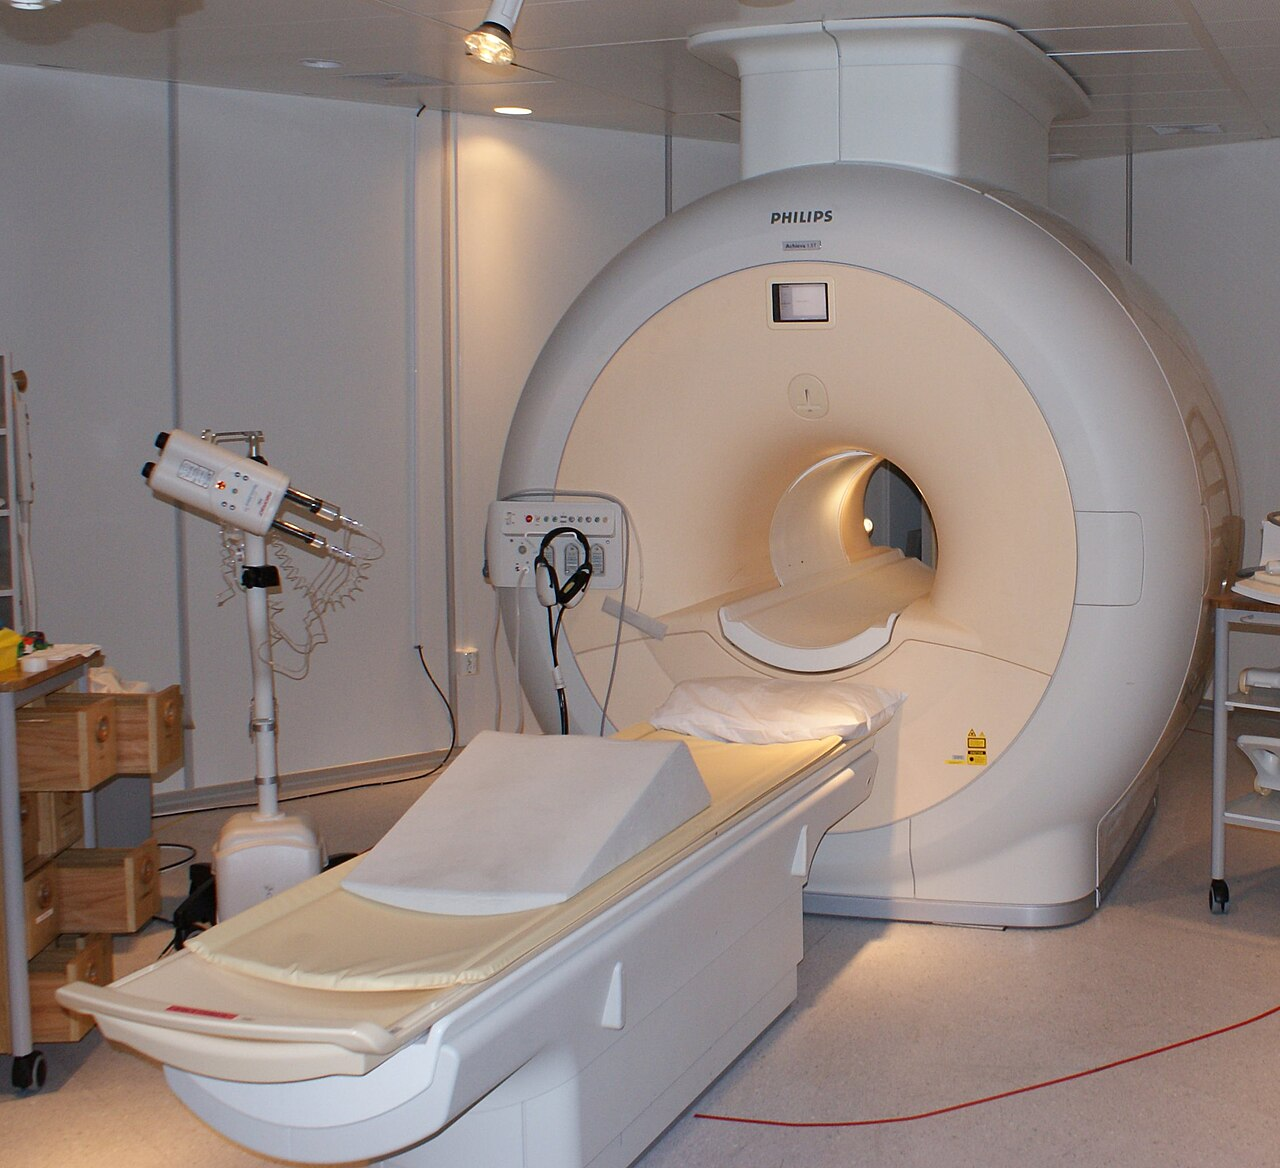
\includegraphics[width=0.50\linewidth]{images/book3/mri-scanner.jpg}

{\small Sebuah pemindai MRI: solenoida superkonduktor yang menahan \qty{1.5}{T} di atas seorang pasien --- satu megajoule \omterm{prop:b1:induction:inductor}{energi magnetik} dalam sebuah medan yang tak berisi apa pun. Foto: Jan Ainali, CC\ BY\ 3.0.}
\end{omfigure}

\section{Hukum Faraday}

\begin{definition}[Fluks magnet menembus sebuah rangkaian]\label{def:b1:induction:flux}
\index{fluks magnet}\index{weber}
Arahkanlah sebuah rangkaian tertutup $\Gamma$ (sebuah arah edar); permukaannya
memperoleh normal $\vect n$ yang diberikan aturan tangan kanan. Yang disebut
\emph{fluks magnet} menembus rangkaiannya adalah $\Phi = \sum\vect B\cdot\vect n\,\dd S$ atas
sebarang permukaan yang dibatasi $\Gamma$ (weber, $\qty{1}{Wb} = \qty{1}{T.m^2}$) ---
``sebarang'', karena fluks $\vect B$ menembus permukaan tertutup bernilai nol.
Bagi medan seragam dan sebuah kumparan datar berlilitan $N$ dan berluas $S$, $\Phi =
NBS\cos\alpha$, dengan $\alpha$ sudut antara $\vect B$ dan $\vect n$.
\end{definition}

\begin{theorem}[Hukum induksi Faraday]\label{thm:b1:induction:faraday}
\index{hukum Faraday}\index{gaya gerak listrik (imbas)}\index{hukum Lenz}
Setiap kali fluks menembus sebuah rangkaian berubah, rangkaiannya menjadi kedudukan
sebuah \emph{\omterm{def:b1:dc-circuits:sources}{gaya gerak listrik} imbas}
\[
e = -\frac{\dd\Phi}{\dd t} ,
\]
yang dihitung dalam arah rangkaiannya, yaitu bekerja sebagai \omterm{def:b1:dc-circuits:sources}{sumber
tegangan} ideal berggl $e$ dalam arah itu; dalam rangkaian berhambatan $R$
ia mengalirkan arus $i = e/R$. Tanda minusnya adalah \emph{\omterm{thm:b1:induction:faraday}{hukum Lenz}}:
arus imbasnya mengalir sedemikian sehingga melawan perubahan fluks yang
menghasilkannya --- medannya sendiri, dan gaya yang dirasakannya, melawan sebabnya.
\end{theorem}
\admitted

\begin{remark}[Dua wajah satu hukum]\label{rem:b1:induction:twofaces}
\index{induksi Neumann}\index{induksi Lorentz}
Fluksnya berubah entah karena $\vect B$ berubah terhadap waktu menembus
rangkaian yang tetap (\emph{\omterm{rem:b1:induction:twofaces}{induksi Neumann}}: transformator, kompor induksi)
atau karena rangkaiannya bergerak atau berubah bentuk dalam medan tunak
(\emph{\omterm{rem:b1:induction:twofaces}{induksi Lorentz}}: generator, \omterm{prop:b1:induction:loudspeaker}{pengeras suara}). Dalam kasus kedua
gglnya dapat pula dihitung langsung: pengemban muatan sebuah unsur penghantar
$\dd\vect l$ yang bergerak dengan $\vect v$ merasakan gaya $q\vect v\wedge
\vect B$, yang setara dengan medan listrik $\vect v\wedge\vect B$, sehingga
$e = \oint(\vect v\wedge\vect B)\cdot\dd\vect l$ --- dan ini selalu sesuai
dengan $-\dd\Phi/\dd t$. \omterm{thm:b1:induction:faraday}{Hukum Faraday} mencakup keduanya; jilid Tahun ke-2
menjelaskan mengapa kedua mekanismenya memberi satu rumus.
\end{remark}

\begin{omfigure}
\begin{tikzpicture}[font=\small, x=1cm, y=1cm, >=Stealth]
  \begin{scope}
    \draw[omThm, very thick, postaction={decorate, decoration={markings, mark=at position 0.25 with {\arrow{>}}, mark=at position 0.75 with {\arrow{>}}}}] (0,0) ellipse (1.4 and 0.5);
    \draw[omDef, thick, ->] (0,0.5) -- (0,1.7) node[right, font=\footnotesize] {$\vect n$};
    \node[omThm, font=\footnotesize] at (1.75,-0.55) {$\Gamma$};
    \foreach \x in {-0.9,-0.3,0.3,0.9} \draw[omProp, ->] (\x,-1.6) -- (\x,1.2);
    \node[omProp, font=\footnotesize] at (1.4,1.05) {$\vect B$};
    \node[font=\footnotesize] at (0,-2.2) {$\Phi = \vect B\cdot\vect n\,S > 0$};
  \end{scope}
  \begin{scope}[xshift=6.2cm]
    \draw[omThm, very thick, postaction={decorate, decoration={markings, mark=at position 0.25 with {\arrow{<}}, mark=at position 0.75 with {\arrow{<}}}}] (0,0) ellipse (1.4 and 0.5);
    \node[omThm, font=\footnotesize] at (1.75,0.6) {$i$};
    % magnet coming down
    \draw[fill=omDef!20, draw=omDef, thick] (-0.4,1.3) rectangle (0.4,2.0); \node[omDef, font=\footnotesize] at (0,1.65) {S};
    \draw[fill=omThm!20, draw=omThm, thick] (-0.4,2.0) rectangle (0.4,2.7); \node[omThm, font=\footnotesize] at (0,2.35) {U};
    \draw[very thick, ->] (0.8,2.6) -- (0.8,1.7) node[right, font=\footnotesize] {$\vect v$};
    \draw[omProp, ->] (0,1.25) -- (0,0.2) node[right, font=\footnotesize, pos=0.6] {$\vect B$ (magnet)};
    \draw[omDef, ->] (-0.6,-0.1) -- (-0.6,0.9) node[left, font=\footnotesize, pos=0.7] {$\vect B_{\text{imb}}$};
    \node[font=\footnotesize] at (0,-2.2) {magnet mendekat: $i$ menolaknya};
  \end{scope}
  \begin{scope}[xshift=11.8cm]
    \draw[omThm, very thick] (-1.4,-0.5) rectangle (1.4,0.5);
    \draw[omThm, very thick] (0.5,-0.5) -- (0.5,0.5);
    \draw[omDef, very thick, ->] (0.5,0.5) -- (0.5,-0.5);
    \draw[very thick, ->] (0.6,0.75) -- (1.2,0.75) node[above, font=\footnotesize] {$\vect v$};
    \foreach \x in {-1.1,-0.6,-0.1,0.4,0.9} \node[omProp, font=\scriptsize] at (\x,0.0) {$\odot$};
    \node[omProp, font=\footnotesize] at (1.75,0.0) {$\vect B$};
    \draw[omDef, ->, thick] (0.5,0.0) -- (-0.2,0.0); \node[omDef, font=\footnotesize] at (-0.15,-0.3) {$\vect F$};
    \node[font=\footnotesize] at (0,-2.2) {batang luncur: fluks tumbuh, $\vect F$ mengerem};
  \end{scope}
\end{tikzpicture}

{\small Arah dan \omterm{thm:b1:induction:faraday}{hukum Lenz}. Kiri: arah rangkaiannya
menetapkan $\vect n$ dan tanda $\Phi$. Tengah: sebuah magnet yang mendekati sebuah
cincin memperbesar fluksnya; arus imbasnya menciptakan medan yang melawan
medan magnetnya dan cincinnya menolaknya. Kanan: sebuah batang yang meluncur pada rel dalam
medan yang menunjuk ke arah pembaca; fluks rangkaiannya tumbuh, dan
arus imbasnya mengalir sehingga \omterm{thm:b1:magnetostatics:laplace}{gaya Laplace} pada batangnya melawan
geraknya.}
\end{omfigure}

\begin{example}[Orde besarnya]\label{ex:b1:induction:orders}
Sebuah kumparan berlilitan $100$ dan berluas \qty{10}{cm^2} dalam medan Bumi, dibalikkan dalam
\qty{0.1}{s}: $\Delta\Phi = 2 \times 100 \times 10^{-3} \times 5 \times 10^{-5} = \qty{1e-5}{Wb}$,
$e \sim \qty{0.1}{mV}$ --- terukur dengan galvanometer yang peka, cara
medan Bumi dahulu dipetakan. Kumparan yang sama dalam celah \qty{1}{T}
sebuah magnet, ditarik keluar dalam \qty{0.1}{s}: \qty{1}{V}. Sebuah kumparan transformator
berlilitan $1000$ dengan \qty{1}{T} pada \qty{50}{Hz} atas \qty{10}{cm^2}: $e_{\max} =
1000 \times 10^{-3} \times 314 = \qty{314}{V}$ --- yaitu listrik jala-jala.
\end{example}

\section{Induktansi diri dan induktansi bersama}

\begin{definition}[Induktansi]\label{def:b1:induction:inductance}
\index{induktansi diri}\index{henry}\index{induktansi bersama}
Fluks medan sebuah rangkaian sendiri yang menembus dirinya sebanding dengan
arusnya: $\Phi_{\text{sendiri}} = Li$, dengan $L > 0$ yang disebut \emph{induktansi diri}-nya
(henry, \unit{H}). Fluks yang dikirim rangkaian~1 menembus rangkaian~2 adalah
$\Phi_{1 \to 2} = Mi_1$, dan secara setangkup $\Phi_{2 \to 1} = Mi_2$, dengan $M$
yang disebut \emph{induktansi bersama}-nya (tandanya ditetapkan oleh arahnya). Maka
fluks total rangkaian~1 adalah $\Phi_1 = L_1i_1 + Mi_2$.
\end{definition}

\begin{proposition}[Induktor; solenoida]\label{prop:b1:induction:inductor}
\index{induktor}\index{energi magnetik}\index{rapat energi medan magnet}
Sebuah rangkaian berinduktansi $L$ yang mengalirkan arus yang berubah menjadi kedudukan
ggl $e = -L\,\dd i/\dd t$: dalam \omterm{thm:b1:dc-circuits:kirchhoff}{kesepakatan penerima} ini adalah
\omterm{def:b1:dc-circuits:voltage}{tegangan} $u = L\,\dd i/\dd t$ induktor yang dipakai sejak
\cref{ch:b1:transient-regimes}. Ia menyimpan energi $W = \tfrac12Li^2$.
Sebuah solenoida panjang berlilitan $n$ tiap meter, panjang $\ell$, penampang $S$,
memiliki $L = \mu_0n^2S\ell$; energi tersimpannya $\tfrac12\mu_0n^2I^2S\ell =
\dfrac{B^2}{2\mu_0}\,S\ell$: \omterm{prop:b1:induction:inductor}{energi magnetik} tinggal di dalam medannya pada
rapat $B^2/2\mu_0$, persis seperti energi listrik pada $\varepsilon_0E^2/2$.
\end{proposition}

\begin{proof}
Faraday dengan $\Phi = Li$, $L$ tetap. Energinya: daya yang diterima
induktornya adalah $ui = Li\,\dd i/\dd t = \dd(\tfrac12Li^2)/\dd t$. Solenoidanya:
$B = \mu_0nI$ di dalam, fluksnya $BS$ menembus tiap lilitan dari $n\ell$ lilitannya, sehingga $\Phi =
\mu_0n^2S\ell I$. Rapat umumnya diterima tanpa bukti.
\end{proof}

\begin{example}[Sebuah magnet MRI]\label{ex:b1:induction:mri}
\qty{1.5}{T} atas kira-kira satu meter kubik: $B^2/2\mu_0 = 2.25/2.5 \times 10^{-6} =
\qty{0.9}{MJ/m^3}$ --- energi sebuah aki mobil, tersimpan dalam ruang kosong.
Dengan arus kumparan \qty{500}{A}, $L = 2W/I^2 = \qty{7}{H}$. Bila
superkonduktornya tiba-tiba menjadi berhambatan (sebuah \emph{padam mendadak}), megajoule itu
menjadi kalor dalam beberapa sekon dan mendidihkan ratusan liter helium
cair: ruang magnetnya memiliki lubang buang untuknya.
\end{example}

\begin{proposition}[Transformator ideal]\label{prop:b1:induction:transformer}
\index{transformator}
Dua kumparan berlilitan $N_1$ dan $N_2$ yang digulung pada teras besi tertutup yang sama,
sehingga fluks $\varphi$ yang sama menembus setiap lilitannya, memenuhi
\[
\frac{u_2}{u_1} = \frac{N_2}{N_1} , \qquad N_1i_1 + N_2i_2 = 0 \quad\text{(tanpa rugi beban, tanpa arus pemagnetan)},
\]
sehingga $u_2i_2 = -u_1i_1$: daya yang diambil pada primernya disalurkan
pada sekundernya; \omterm{def:b1:dc-circuits:voltage}{tegangannya} berjenjang menurut nisbah lilitan, arusnya
berbanding terbalik. Ia hanya bekerja dengan arus yang berubah.
\end{proposition}

\begin{proof}
$u_1 = N_1\,\dd\varphi/\dd t$ dan $u_2 = N_2\,\dd\varphi/\dd t$ (\omterm{thm:b1:dc-circuits:kirchhoff}{kesepakatan
penerima} pada keduanya, arahnya dipilih menyusuri fluks bersamanya): bagilah.
Hubungan arusnya adalah \omterm{thm:b1:magnetostatics:ampere}{hukum Ampère} pada terasnya: sirkulasinya
sebesar $\mu_0\mu_r$ kali ampere-lilitan totalnya harus menciptakan
fluksnya; bagi teras ideal ($\mu_r \to \infty$) itu menuntut ampere-lilitan
yang lenyap, sehingga $N_1i_1 + N_2i_2 = 0$. Diterima tanpa bukti dalam bentuk ini.
\end{proof}

\begin{omfigure}
\begin{tikzpicture}[font=\small, x=1cm, y=1cm, >=Stealth]
  % core
  \draw[omExo!60, line width=9pt] (-2,-1.5) rectangle (2,1.5);
  % primary windings
  \foreach \y in {-0.9,-0.6,...,0.9} \draw[omThm, thick] (-2.35,\y) arc[start angle=90, end angle=-90, x radius=0.18, y radius=0.15];
  \foreach \y in {-0.9,-0.6,...,0.9} \draw[omDef, thick] (2.35,\y) arc[start angle=90, end angle=270, x radius=0.18, y radius=0.15];
  \draw[omThm, thick] (-2.35,0.9) -- (-3.2,0.9) node[left, font=\footnotesize] {$u_1$}; \draw[omThm, thick] (-2.35,-1.2) -- (-3.2,-1.2);
  \draw[omDef, thick] (2.35,0.9) -- (3.2,0.9) node[right, font=\footnotesize] {$u_2$}; \draw[omDef, thick] (2.35,-1.2) -- (3.2,-1.2);
  \node[omThm, font=\footnotesize] at (-2.9,0) {$N_1$}; \node[omDef, font=\footnotesize] at (2.9,0) {$N_2$};
  \draw[omProp, thick, dashed, ->] (-1.3,-0.9) -- (-1.3,0.9) -- (1.3,0.9) -- (1.3,-0.9) -- cycle;
  \node[omProp, font=\footnotesize] at (0,0) {fluks $\varphi$};
  \node[font=\footnotesize] at (0,-2.2) {$u_2/u_1 = N_2/N_1$, \quad $N_1 i_1 = -N_2 i_2$};
  \begin{scope}[xshift=8.6cm]
    \draw[omThm, very thick] (-1.6,0) -- (1.6,0);
    \foreach \x in {-1.3,-0.9,...,1.3} \draw[omThm, thick] (\x,0) arc[start angle=180, end angle=0, x radius=0.2, y radius=0.45];
    \draw[omDef, very thick] (-1.2,-1.1) -- (1.2,-1.1);
    \foreach \x in {-0.9,-0.5,...,0.9} \draw[omDef, thick] (\x,-1.1) arc[start angle=180, end angle=0, x radius=0.2, y radius=0.35];
    \node[omThm, font=\footnotesize] at (-2.1,0.3) {$i_1$, $L_1$}; \node[omDef, font=\footnotesize] at (-1.9,-0.9) {$L_2$};
    \draw[<->, omProp] (0,0.7) -- (0,-0.9) node[midway, right, font=\footnotesize] {$M$};
    \node[font=\footnotesize] at (0,-2.2) {$\Phi_1 = L_1 i_1 + M i_2$};
  \end{scope}
\end{tikzpicture}

{\small Kiri: sebuah transformator --- dua kumparan pada teras besi tertutup berbagi
fluks yang sama; \omterm{def:b1:dc-circuits:voltage}{tegangannya} berskala menurut lilitannya, arusnya
berbanding terbalik. Kanan: dua kumparan terkopel di udara dan \omterm{def:b1:induction:inductance}{induktansi
bersamanya} $M$; fluks sebuah kumparan sendiri adalah $Li$.}
\end{omfigure}

\section{Penghantar yang bergerak: generator dan motor}

\begin{proposition}[Batang luncur]\label{prop:b1:induction:rails}
\index{rel Laplace}\index{konversi elektromekanis}
Sebuah batang sepanjang $\ell$ meluncur dengan kelajuan $v$ pada dua rel yang ditutup
sebuah hambatan $R$, dalam medan seragam $B$ yang normal terhadap bidangnya. Ia menjadi
kedudukan ggl $e = B\ell v$, mengalirkan $i = B\ell v/R$, dan merasakan
\omterm{thm:b1:magnetostatics:laplace}{gaya Laplace} $F = B\ell i = B^2\ell^2v/R$ yang \emph{melawan} geraknya.
Daya mekanis yang dikeluarkan untuk mendorongnya, $Fv$, sama dengan \omterm{thm:b1:dc-circuits:kirchhoff}{daya listrik}
$ei = Ri^2$ yang dilesapkan: batangnya adalah sebuah generator. Bila sebaliknya diberi
sumber $E$, ia menjadi motor: arus $(E - B\ell v)/R$ mendorongnya
sampai ggl baliknya $B\ell v$ mengimbangi $E$, pada kelajuan tanpa beban $E/B\ell$.
\end{proposition}

\begin{proof}
Fluksnya $B\ell x$, $e = -B\ell\dot x$ dalam arah yang membuat $\vect n$
menyusuri $\vect B$; \omterm{thm:b1:magnetostatics:laplace}{gaya Laplace} $i\vect\ell\wedge\vect B$ pada arus
yang berarah demikian menunjuk melawan $\vect v$ (\cref{thm:b1:induction:faraday},
Lenz). Kalikanlah persamaan listriknya $e = Ri$ dengan $i$ dan persamaan
mekanisnya dengan $v$: $Fv = B\ell iv = ei$. Daya elektromekanis
$ei$ dan daya Laplace $-Fv$ selalu berlawanan --- itulah hukum
konversinya.
\end{proof}

\begin{proposition}[Lilitan yang berputar: alternator]\label{prop:b1:induction:alternator}
\index{alternator}
Sebuah kumparan berlilitan $N$ dan berluas $S$ yang berputar dengan $\omega$ terhadap sumbu
yang tegak lurus pada $B$ yang seragam memiliki $\Phi = NBS\cos\omega t$ dan
\[
e = NBS\omega\sin\omega t :
\]
yaitu sebuah ggl sinusoidal beramplitudo $NBS\omega$ dan berfrekuensi putarnya.
Ke dalam sebuah hambatan $R$ ia menyalurkan \omterm{thm:b1:sinusoidal-impedance:power}{daya rata-rata} $(NBS\omega)^2/2R$,
yang dipasok oleh \omterm{def:b1:angular-momentum:moment}{momen gaya} yang menjaganya tetap berputar melawan kopel
Laplace $-\vect m\wedge\vect B$ arusnya sendiri.
\end{proposition}

\begin{proof}
Turunkanlah fluksnya; $\langle\sin^2\rangle = \tfrac12$. Kopelnya adalah
\cref{thm:b1:magnetostatics:dipoleinfield} dengan $m = Ni S$; \omterm{thm:b1:sinusoidal-impedance:power}{daya
rata-ratanya} $\langle\Gamma\omega\rangle$ sama dengan $\langle ei\rangle$ menurut perhitungan
yang sama seperti bagi batangnya.
\end{proof}

\begin{omfigure}
\begin{tikzpicture}[font=\small, x=1cm, y=1cm, >=Stealth]
  \begin{scope}
    \draw[omThm, very thick] (-1.8,-1.0) -- (1.8,-1.0); \draw[omThm, very thick] (-1.8,1.0) -- (1.8,1.0);
    \draw[omThm, very thick] (-1.8,-1.0) -- (-1.8,1.0);
    \draw[omDef, very thick] (0.8,-1.0) -- (0.8,1.0);
    \draw[omDef, very thick, ->] (0.8,-0.2) -- (0.8,0.3) node[right, font=\footnotesize] {$i$};
    \draw[omProp, thick, ->] (0.8,0) -- (0.05,0) node[above, font=\footnotesize, pos=0.5] {$\vect F$};
    \draw[very thick, ->] (1.0,1.25) -- (1.7,1.25) node[right, font=\footnotesize] {$\vect v$};
    \foreach \x in {-1.4,-0.9,-0.4,0.1,1.3} \foreach \y in {-0.5,0.5} \node[omProp, font=\scriptsize] at (\x,\y) {$\odot$};
    \draw[fill=white] (-1.95,-0.35) rectangle (-1.65,0.35); \node[font=\footnotesize] at (-2.45,0) {$R$};
    \node[font=\footnotesize] at (0,-1.6) {$e = B\ell v$, \; $F = B^2\ell^2 v/R$};
  \end{scope}
  \begin{scope}[xshift=6.5cm]
    \draw[omThm, very thick, rotate=30] (-1.2,-0.6) rectangle (1.2,0.6);
    \draw[dashed] (0,-1.6) -- (0,1.6); \node[font=\footnotesize] at (0,1.85) {sumbu};
    \foreach \y in {-1.2,-0.6,0,0.6,1.2} \draw[omProp, ->] (-2.2,\y) -- (2.2,\y);
    \node[omProp, font=\footnotesize] at (2.0,1.45) {$\vect B$};
    \draw[->, very thick] (0,0) -- (120:1.0) node[above left, font=\footnotesize] {$\vect n$};
    \draw (0.6,0) arc[start angle=0, end angle=120, radius=0.6] node[midway, above right, font=\footnotesize] {$\omega t$};
    \node[font=\footnotesize] at (0,-2.0) {$\Phi = NBS\cos\omega t$, \; $e = NBS\omega\sin\omega t$};
  \end{scope}
\end{tikzpicture}\hfill
\begin{tikzpicture}
\begin{axis}[omaxis, axis x line=middle, axis y line=left, width=4.3cm, height=3.8cm,
    xlabel={$t$}, ylabel={$e$}, xmin=0, xmax=6.6, ymin=-1.3, ymax=1.3, xtick=\empty, ytick=\empty, samples=80,
    xlabel style={at={(axis description cs:1.0,0.55)}, anchor=west}]
  \addplot[omDef, thick, domain=0:6.28] {sin(deg(x))};
\end{axis}
\end{tikzpicture}

{\small Kiri: batang luncur sebagai generator --- ggl $B\ell v$, arus
lewat $R$, \omterm{thm:b1:magnetostatics:laplace}{gaya Laplace} yang mengerem batangnya; daya pendorongnya menjadi
kalor \omterm{def:b1:dc-circuits:resistor}{resistornya}. Tengah dan kanan: kumparan berputar sebuah alternator
dan ggl sinusoidalnya.}
\end{omfigure}

\begin{example}[Arus pusar]\label{ex:b1:induction:eddy}
\index{arus pusar}
Sebuah penghantar pejal yang bergerak dalam medan tak seragam, atau yang duduk dalam
medan yang berubah, ditembus fluks yang berubah menyusuri \omterm{def:b1:point-kinematics:frame}{lintasan} tertutup yang tak terhitung:
\emph{\omterm{ex:b1:induction:eddy}{arus pusar}} beredar di dalamnya, memanaskannya dan --- menurut Lenz ---
mengeremnya. Sebuah magnet yang dijatuhkan ke dalam tabung tembaga melayang turun perlahan;
rem truk dan kereta luncur memakainya (tanpa sentuhan, tanpa aus, tanpa
kegagalan rem --- tetapi tanpa pengereman saat diam); kompor induksi memanaskan
pancinya dengan arus yang sama, pada \qty{25}{kHz}; teras transformator
dilapis-lapiskan justru untuk memutusnya.
\end{example}

\section{Pengeras suara: sebuah sistem terkopel}

\begin{proposition}[Kopling elektromekanis sebuah kumparan dalam medan radial]\label{prop:b1:induction:loudspeaker}
\index{pengeras suara}\index{mikrofon}
Sebuah kumparan yang panjang kawat totalnya $\ell$ duduk dalam medan radial $B$ sehingga
setiap unsur kawatnya tegak lurus pada $\vect B$; ia bergerak menyusuri
sumbunya dengan kelajuan $v$ dan mengalirkan $i$. Maka ia merasakan \omterm{thm:b1:magnetostatics:laplace}{gaya Laplace} aksial
$F = B\ell i$ dan menjadi kedudukan ggl balik $e = -B\ell v$ (\omterm{thm:b1:dc-circuits:kirchhoff}{kesepakatan
penerima}: \omterm{def:b1:dc-circuits:voltage}{tegangan} $B\ell v$). Dengan massa $m$, gantungan
berkekakuan $k$ dan peredaman mekanis $h$, yang diberi \omterm{def:b1:dc-circuits:voltage}{tegangan} $u$ lewat
hambatan $R$ dan induktansi $L$ kumparannya:
\[
u = Ri + L\frac{\dd i}{\dd t} + B\ell v , \qquad
m\frac{\dd v}{\dd t} = -kx - hv + B\ell i .
\]
Dikalikan $i$ dan $v$ lalu dijumlahkan: \omterm{thm:b1:dc-circuits:kirchhoff}{daya listrik} $ui$
sama dengan rugi Joule $Ri^2$ ditambah pertumbuhan energi tersimpannya
$\tfrac12Li^2 + \tfrac12mv^2 + \tfrac12kx^2$ ditambah rugi mekanisnya
$hv^2$ (yang mencakup bunyinya): suku konversinya $B\ell iv$ saling meniadakan
antara kedua persamaannya. Dijalankan terbalik (geraknya dipaksakan, $u$ dibaca)
peranti yang sama menjadi sebuah \emph{mikrofon} dinamik.
\end{proposition}

\begin{proof}
\omterm{thm:b1:magnetostatics:laplace}{Gaya Laplace} pada tiap unsurnya $i\,\dd\vect l\wedge\vect B$, semuanya aksial dan
bertanda sama; gglnya dari $(\vect v\wedge\vect B)\cdot\dd\vect l$ yang dijumlahkan
atas kawatnya. Neraca energinya adalah jumlah kedua persamaannya
yang dikalikan seperti dinyatakan.
\end{proof}

\begin{omfigure}
\begin{tikzpicture}[font=\small, x=1cm, y=1cm, >=Stealth]
  % magnet structure (cross-section)
  \draw[fill=omExo!30, draw=omExo, thick] (-3.0,-1.2) rectangle (-0.6,1.2);
  \draw[fill=omExo!30, draw=omExo, thick] (-0.6,-0.35) rectangle (1.6,0.35);
  \draw[fill=omExo!30, draw=omExo, thick] (-0.6,0.85) rectangle (1.6,1.2);
  \draw[fill=omExo!30, draw=omExo, thick] (-0.6,-1.2) rectangle (1.6,-0.85);
  \node[omExo, font=\footnotesize] at (-1.8,0) {magnet};
  % coil in the gaps
  \foreach \x in {0.9,1.05,1.2,1.35} {\fill[omThm] (\x,0.6) circle (1.6pt); \fill[omThm] (\x,-0.6) circle (1.6pt);}
  \node[omThm, font=\footnotesize] at (1.1,1.55) {kumparan suara};
  % radial field arrows in the gaps
  \foreach \x in {0.3,0.55} {\draw[omProp, ->] (\x,0.4) -- (\x,0.8); \draw[omProp, ->] (\x,-0.4) -- (\x,-0.8);}
  \node[omProp, font=\footnotesize] at (-0.2,0.6) {$\vect B$};
  % cone
  \draw[thick] (1.6,0.6) -- (3.4,2.2); \draw[thick] (1.6,-0.6) -- (3.4,-2.2);
  \draw[thick] (1.6,0.6) -- (1.6,-0.6);
  \node[font=\footnotesize] at (2.9,-0.95) {kerucut, $m$};
  \draw[thick, decorate, decoration={coil, aspect=0.6, segment length=3pt, amplitude=2pt}] (3.4,2.2) -- (3.4,2.9); \draw[thick] (3.0,2.9) -- (3.8,2.9);
  \draw[thick, decorate, decoration={coil, aspect=0.6, segment length=3pt, amplitude=2pt}] (3.4,-2.2) -- (3.4,-2.9); \draw[thick] (3.0,-2.9) -- (3.8,-2.9);
  \node[font=\footnotesize] at (3.4,3.25) {gantungan $k$, $h$};
  \draw[omDef, very thick, ->] (1.6,0) -- (2.6,0);
  \node[omDef, font=\footnotesize, anchor=south west] at (1.75,0.08) {$F = B\ell i$};
  \draw[very thick, ->] (4.6,0.5) -- (5.6,0.5) node[right, font=\footnotesize] {$v$};
  \node[font=\footnotesize] at (5.3,-1.7) {$u = Ri + L\frac{\dd i}{\dd t} + B\ell v$};
\end{tikzpicture}

{\small Sebuah \omterm{prop:b1:induction:loudspeaker}{pengeras suara} kumparan bergerak dalam penampang: kumparan suaranya duduk di
celah gelang sebuah magnet yang medannya radial, sehingga sebuah
arus memberi gaya aksial apa pun kedudukannya; kerucut yang digeraknya
ditahan oleh gantungan yang kaku dan teredam; gerak kumparannya memberi
ggl balik $B\ell v$ ke dalam rangkaian listriknya.}
\end{omfigure}

\begin{remark}[Mengapa koplingnya meredam]\label{rem:b1:induction:damping}
Pada frekuensi rendah ($L\omega \ll R$), $i \approx (u - B\ell v)/R$ dan gayanya
adalah $B\ell u/R - (B^2\ell^2/R)\,v$: rangkaian listriknya menambahkan peredaman
$B^2\ell^2/R$ pada peredaman mekanisnya. Sebuah \omterm{prop:b1:induction:loudspeaker}{pengeras suara} yang tersambung ke
penguat (berhambatan keluaran rendah) teredam berat --- kerucutnya berhenti
ketika \omterm{def:b1:wave-propagation:signal}{sinyalnya} berhenti --- dan kopling yang sama pula yang membuat
mikrofonnya mengambil energi dari bunyinya (\cref{pb:b1:induction:1}).
\end{remark}

\section{Latihan}

\begin{exercise}[$\star$]\label{exo:b1:induction:1}
Sebuah kumparan berlilitan $100$ dan berluas \qty{10}{cm^2} dalam medan seragam \qty{0.20}{T} bersudut
\qty{30}{\degree} terhadap normalnya. Fluksnya; ggl rata-rata bila medannya dimatikan
dalam \qty{10}{ms}; dalam \qty{1}{ms}; arah arus imbasnya
relatif terhadap medannya (Lenz).
\end{exercise}

\begin{exercise}[$\star$]\label{exo:b1:induction:2}
Sebuah batang sepanjang \qty{20}{cm} meluncur dengan \qty{2.0}{m/s} pada rel yang ditutup
\qty{0.10}{\ohm}, dalam \qty{0.50}{T}. Ggl, arus, \omterm{thm:b1:magnetostatics:laplace}{gaya Laplace}, gaya yang harus
dikerahkan pendorongnya, daya mekanis, \omterm{thm:b1:dc-circuits:kirchhoff}{daya listriknya}.
\end{exercise}

\begin{exercise}[$\star$]\label{exo:b1:induction:3}
Solenoida \qty{1000}{lilitan/m}, panjang \qty{20}{cm}, penampang \qty{4.0}{cm^2}:
induktansinya; energinya pada \qty{5.0}{A}; \omterm{def:b1:transient-regimes:firstorder}{tetapan waktunya} dengan hambatan
\qty{1.0}{\ohm}; medan di dalamnya dan rapat energinya, untuk memeriksa $B^2/2\mu_0$.
\end{exercise}

\begin{exercise}[$\star$]\label{exo:b1:induction:4}
Sebuah transformator dari \qty{230}{V} ke \qty{12}{V}: nisbah lilitannya; lilitan
primernya bagi sekunder berlilitan $50$; arus primernya ketika sekundernya
menyalurkan \qty{2.0}{A}. Mengapa ia tak bekerja pada aki mobil?
\end{exercise}

\begin{exercise}[$\star\star$]\label{exo:b1:induction:5}
\omterm{thm:b1:induction:faraday}{Hukum Lenz}: berikanlah arah arus imbasnya dan arah
gayanya pada tiap kasus --- (a) sebuah kutub utara mendekati sebuah cincin menyusuri
sumbunya; (b) sebuah cincin terletak dalam medan yang tumbuh; (c) sebuah cincin dijatuhkan
ke atas sebuah magnet; (d) sebuah magnet jatuh menembus tabung tembaga yang panjang. Bagi (d),
jelaskanlah dengan energi mengapa ia jatuh dengan kelajuan tetap yang kecil.
\end{exercise}

\begin{exercise}[$\star\star$]\label{exo:b1:induction:6}
Alternator: $N = 200$, $S = \qty{20}{cm^2}$, $B = \qty{0.10}{T}$, \qty{50}{Hz}.
Ggl puncak dan rms-nya; arus puncak dan \omterm{def:b1:angular-momentum:moment}{momen gaya} puncak ke dalam \qty{10}{\ohm}; \omterm{thm:b1:dc-circuits:kirchhoff}{daya
listrik} rata-ratanya; bandingkan dengan daya mekanis rata-ratanya, dan dengan
\omterm{def:b1:angular-momentum:moment}{momen gaya} sesaat pada saat gglnya lenyap.
\end{exercise}

\begin{exercise}[$\star\star$]\label{exo:b1:induction:7}
\emph{Rem magnetik.} Sebuah lilitan persegi bersisi $a = \qty{10}{cm}$ dan
berhambatan $R = \qty{1.0}{m\ohm}$, bermassa \qty{1.0}{kg}, meninggalkan sebuah daerah
bermedan seragam $B = \qty{1.0}{T}$ dengan kelajuan $v$ (satu sisinya masih di dalam
medannya). Ggl, arus, gaya pengeremnya; persamaan gerak dan \omterm{def:b1:transient-regimes:firstorder}{tetapan
waktunya}; jarak yang ditempuh sebelum berhenti dari \qty{1.0}{m/s}; ke mana
\omterm{thm:b1:work-and-energy:ke}{energi kinetiknya} pergi?
\end{exercise}

\begin{exercise}[$\star\star$]\label{exo:b1:induction:8}
Sebuah kumparan kecil ($N_2 = 50$ lilitan, penampang \qty{2.0}{cm^2}) duduk di dalam
sebuah solenoida panjang ($n_1 = \qty{2000}{m^{-1}}$), sumbunya sejajar. \omterm{def:b1:induction:inductance}{Induktansi
bersamanya}; ggl dalam kumparannya ketika arus solenoidanya menanjak
\qty{100}{A/s}, dan ketika arusnya $\qty{1.0}{A}$ pada \qty{10}{kHz}. Apakah $M$
bergantung pada kumparan mana yang mengalirkan arusnya?
\end{exercise}

\begin{exercise}[$\star\star$]\label{exo:b1:induction:9}
\omterm{def:b1:kinetic-theory:U}{Energi dalam} sebuah medan: $B = \qty{1.5}{T}$ atas \qty{1.0}{m^3}, seperti dalam sebuah magnet
MRI. Energinya; induktansinya bagi $I = \qty{500}{A}$; ketinggian yang dapat dinaiki
sebuah mobil \qty{1}{t} dengan energi itu; volume helium cair yang dididihkannya
dalam sebuah padam mendadak (\qty{2.6}{kJ} tiap liter). Energi medan Bumi
(\qty{5e-5}{T}) dalam sebuah ruangan \qty{50}{m^3}.
\end{exercise}

\begin{exercise}[$\star\star\star$]\label{exo:b1:induction:10}
\emph{Rel sebagai motor.} Batang \cref{exo:b1:induction:2} (bermassa $m$,
tanpa gesekan) dihubungkan ke sumber $E$ lewat hambatan $R$.
(a) Persamaan listrik dan mekanisnya; tunjukkan $m\,\dd v/\dd t = B\ell(E -
B\ell v)/R$. (b) Kelajuan terminal dan \omterm{def:b1:transient-regimes:firstorder}{tetapan waktunya}. (c) Neraca daya:
daya sumber $=$ Joule $+$ mekanis; \omterm{def:b1:heat-engines:efficiency}{efisiensinya} sebagai fungsi
$v$. (d) Angkanya: $E = \qty{2.0}{V}$, $m = \qty{50}{g}$, sisanya seperti dalam
\cref{exo:b1:induction:2}. (e) Sebuah senapan rel mempercepat proyektil
\qty{10}{g} dengan \qty{1}{MA} sepanjang \qty{5}{m} dalam \qty{1}{T}: kelajuan keluarnya
(\omterm{def:b1:units-dimensions:oom}{orde besarnya}).
\end{exercise}

\begin{exercise}[$\star\star\star$]\label{exo:b1:induction:11}
\emph{Cakram Faraday.} Sebuah cakram tembaga berjari-jari $R$ berputar dengan $\omega$
terhadap sumbunya dalam $B$ seragam yang menyusuri sumbunya; sikatnya menyentuh pusatnya
dan tepinya. (a) Ggl antara pusat dan tepinya dengan menjumlahkan $(\vect v\wedge
\vect B)\cdot\dd\vect l$ menyusuri sebuah jari-jari: $e = \tfrac12B\omega R^2$. (b) Angkanya:
$R = \qty{10}{cm}$, \qty{3000}{rpm}, \qty{1.0}{T}. (c) Mengapa ia mesin
bertegangan rendah dan berarus tinggi; arusnya ke dalam \qty{1}{m\ohm}, dan
\omterm{def:b1:angular-momentum:moment}{momen gaya} pengeremnya. (d) Perolehlah kembali $e$ dari \omterm{thm:b1:induction:faraday}{hukum Faraday} yang diterapkan pada
rangkaian sikat--jari-jari--tepi--sikat: fluks mana yang berubah?
\end{exercise}

\begin{exercise}[$\star\star\star$]\label{exo:b1:induction:12}
\emph{Kompor induksi.} Kumparan di bawah kacanya mengalirkan $i_1 =
I_1\cos\omega t$ dengan $I_1 = \qty{30}{A}$ pada \qty{25}{kHz}; dasar pancinya
berlaku sebagai satu lilitan berhambatan $R_p = \qty{10}{m\ohm}$ yang terkopel oleh
$M = \qty{1.0}{\micro H}$ (induktansi lilitan pancinya diabaikan). (a) Ggl
yang terimbas pada pancinya, nilai puncaknya. (b) Arus dan \omterm{thm:b1:sinusoidal-impedance:power}{daya rata-rata} yang dilesapkan
pada pancinya. (c) Mengapa frekuensinya tinggi, dan mengapa kalornya muncul pada
pancinya dan bukan pada kacanya? (d) Arus pancinya berbalik bekerja pada kumparannya:
ggl yang diimbaskannya di sana (puncak), dan daya tambahan yang harus dipasok
generatornya --- periksalah bahwa ia sama dengan (b).
\end{exercise}

\begin{omfigure}
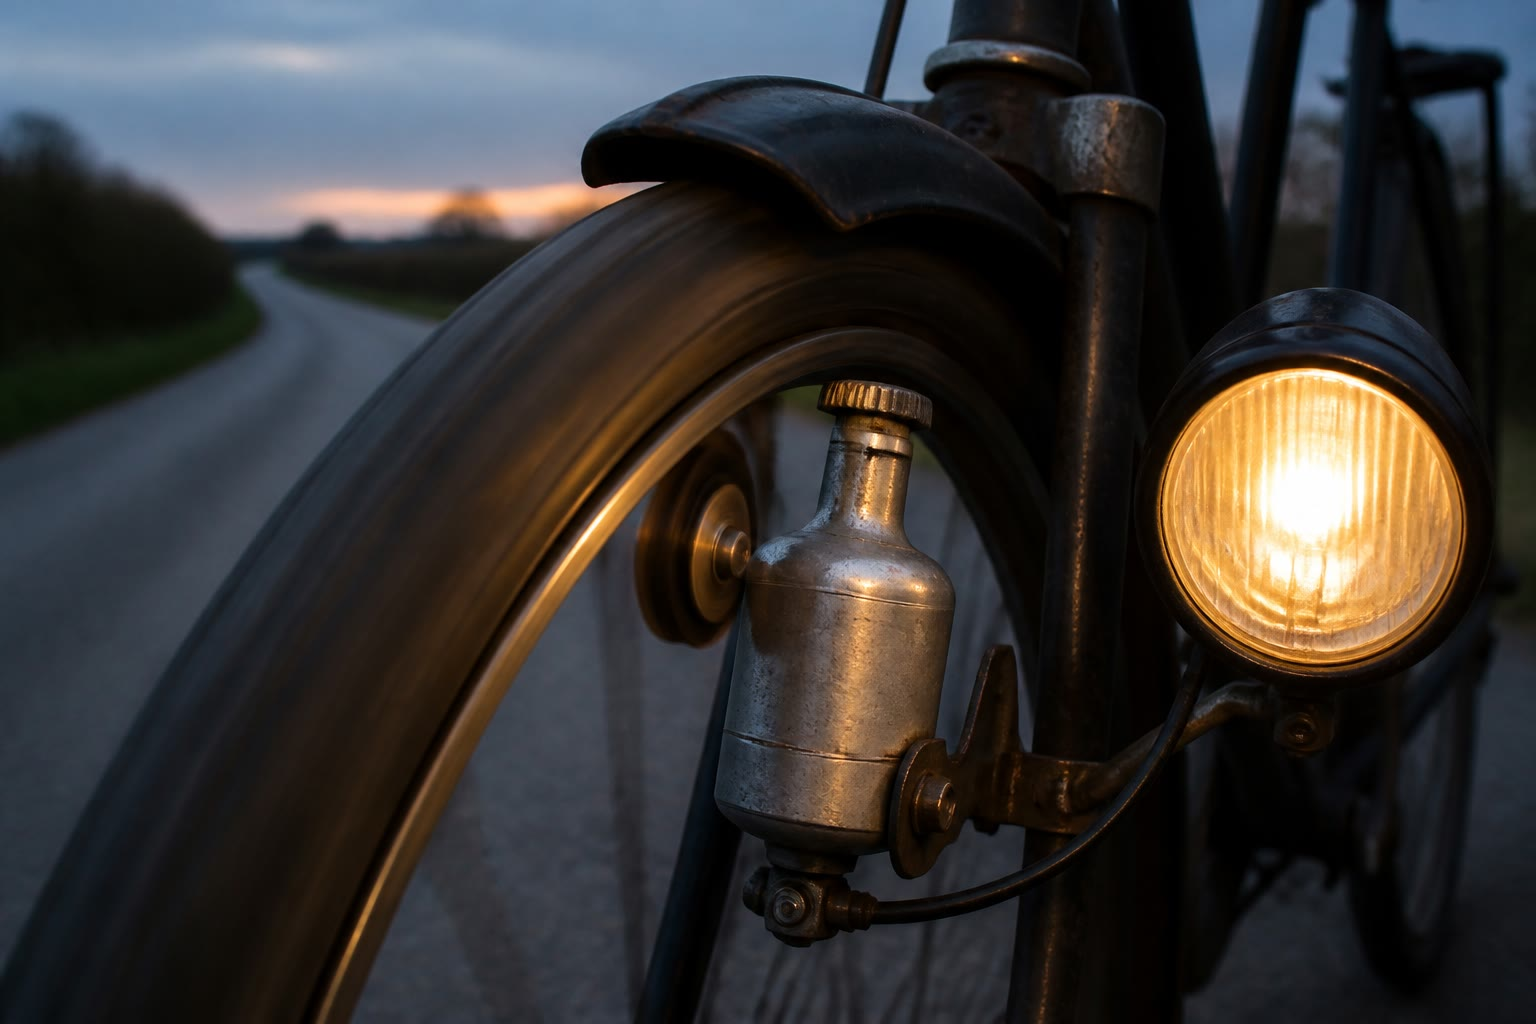
\includegraphics[width=0.58\linewidth]{images/book3/ai/b3-29-bicycle-dynamo.jpg}

{\small Sebuah dinamo botol: rodanya memutar sebuah magnet di dalam sebuah kumparan, fluks yang menembus kumparannya berubah, dan lampunya menyala --- \omterm{thm:b1:induction:faraday}{hukum Faraday} di atas sebuah sepeda.}
\end{omfigure}

\section{Soal: Dinamo sepeda dan pengeras suara}

\begin{problem}[{Soal akhir pekan --- dua pengubah elektromekanis
yang dibongkar: sebuah dinamo yang mengatur dirinya sendiri, dan sebuah pengeras suara
yang penguatnya sekaligus remnya}]
\label{pb:b1:induction:1}

\medskip
\noindent\textbf{Bagian I --- Dinamo sepedanya.}
Sebuah kumparan berlilitan $N = 300$ dan berluas $S = \qty{3.0}{cm^2}$ berputar dalam
medan seragam $B = \qty{0.30}{T}$; porosnya membawa sebuah rol berjari-jari
$r = \qty{1.0}{cm}$ yang ditekan pada bannya, sehingga kumparannya berputar dengan
$\omega = v/r$ bagi kelajuan sepeda $v$. Hambatan kumparannya $r_c = \qty{4.0}{\ohm}$,
induktansinya $L = \qty{20}{mH}$; lampunya adalah hambatan $R = \qty{12}{\ohm}$.
\begin{enumerate}
  \item Fluks menembus kumparannya dan ggl imbasnya sebagai fungsi waktu;
        \omterm{def:b1:wave-propagation:signal}{amplitudo} dan frekuensinya pada $v = \qty{18}{km/h}$.
  \item Dengan mengabaikan $L$ dahulu: arus rms dan daya pada lampunya pada
        \qty{18}{km/h}; apakah lampu ``\qty{6}{V}, \qty{3}{W}'' merasa nyaman?
  \item Daya mekanis rata-rata yang dipasok pengendaranya ke dinamonya, dan
        gaya yang bersesuaian pada bannya (bandingkan dengan gesekan
        gelinding, kira-kira \qty{2}{N}).
  \item Jelaskanlah dengan \omterm{thm:b1:induction:faraday}{hukum Lenz} mengapa dinamonya melawan, dan mengapa sebuah lampu
        yang menyala ``cuma-cuma'' tak bertentangan dengan kekekalan energi.
  \item Kini sertakanlah $L$: impedans kompleks rangkaiannya; tunjukkan bahwa
        \omterm{def:b1:wave-propagation:signal}{amplitudo} arusnya adalah $I = NBS\omega/\sqrt{(R + r_c)^2 + L^2\omega^2}$
        dan bahwa ia menjenuh pada kelajuan tinggi; limitnya, dan
        kelajuan saat ia mencapai $70\%$ limitnya.
  \item Tanpa induktansinya, apa yang akan diterima lampunya pada
        \qty{54}{km/h} menuruni bukit? Dengan induktansinya?
  \item Arus dan daya lampunya pada \qty{9}{km/h} dan pada \qty{36}{km/h}; ulaslah
        pengaturan dirinya.
  \item Dinamo yang sebenarnya memutar sebuah magnet di dalam kumparan yang tetap. Apakah
        analisisnya berubah? Masalah praktis apa yang disingkirkannya?
  \item Apa yang dilakukan lampunya ketika sepedanya berhenti di lampu merah,
        dan bagaimana lampu modern mengatasinya?
\end{enumerate}

\medskip
\noindent\textbf{Bagian II --- \omterm{prop:b1:induction:loudspeaker}{Pengeras suaranya}.}
Kumparan suaranya: panjang kawat $\ell = \qty{5.0}{m}$ dalam medan radial $B =
\qty{1.0}{T}$, hambatan $R = \qty{8.0}{\ohm}$, induktansi $L = \qty{0.50}{mH}$;
massa bergeraknya (kumparan dan kerucut) $m = \qty{10}{g}$; kekakuan gantungannya
$k = \qty{1000}{N/m}$, peredaman mekanisnya $h = \qty{1.0}{N.s/m}$. Rezim
sinusoidal, \omterm{def:b1:sinusoidal-impedance:complex}{amplitudo kompleks}.
\begin{enumerate}[resume]
  \item Gaya pada kumparannya bagi arus $i$; ggl baliknya bagi kelajuan $v$
        (turunkanlah keduanya, lengkap dengan tandanya).
  \item Tuliskanlah persamaan listrik dan mekanisnya.
  \item Hapuskanlah $i$ lalu tunjukkan bahwa
        $\underline v = \dfrac{B\ell\,\underline u}{(R + jL\omega)(jm\omega + h + k/j\omega) + B^2\ell^2}$.
  \item Pada frekuensi yang $L\omega \ll R$, tunjukkan bahwa koplingnya bekerja
        sebagai peredaman mekanis tambahan $B^2\ell^2/R$; nilainya; frekuensi
        resonansi kerucutnya dan faktor kualitasnya dengan dan tanpa
        peredaman listriknya.
  \item Penguatnya menyalurkan $i$ beramplitudo \qty{1.0}{A} pada \qty{1}{kHz}:
        \omterm{def:b1:wave-propagation:signal}{amplitudo} gaya, percepatan, perpindahan dan kecepatan
        kerucutnya (rezim terkendali massa); \omterm{def:b1:wave-propagation:signal}{amplitudo} ggl baliknya dibandingkan dengan
        $Ri$.
  \item Arus yang sama pada frekuensi resonansinya: \omterm{def:b1:wave-propagation:signal}{amplitudo} kecepatannya
        (terkendali peredaman) dan ggl baliknya; ulaslah.
  \item \omterm{thm:b1:dc-circuits:kirchhoff}{Daya listriknya} pada \qty{1}{kHz}; daya mekanis yang dilesapkan pada
        $h$ (diambil sebagai rugi bunyi dan gantungannya); \omterm{def:b1:heat-engines:efficiency}{efisiensinya}.
  \item Mengapa tekanan bunyinya sebanding dengan percepatan
        kerucutnya (terimalah tanpa bukti) menjadi sebab kerucut yang terkendali massa memberi
        tanggapan yang datar di atas resonansinya?
  \item Mengapa medannya harus radial, dan mengapa sebuah tweeter berukuran kecil?
  \item Sketsalah modulus impedans $\underline u/\underline i$ yang terlihat
        oleh penguatnya dari \qty{10}{Hz} sampai \qty{10}{kHz}: nilainya pada frekuensi
        rendah, pada resonansinya (pakailah kecepatan yang terkendali peredaman),
        dan pada \qty{10}{kHz}.
\end{enumerate}

\medskip
\noindent\textbf{Bagian III --- Terbalik, dan bukunya.}
\begin{enumerate}[resume]
  \item Peranti yang sama sebagai mikrofon: sebuah bunyi menggerakkan kerucutnya dengan
        $v = \qty{1.0}{mm/s}$; \omterm{def:b1:dc-circuits:voltage}{tegangan} rangkaian terbukanya.
  \item Dibebani $R_L = \qty{600}{\ohm}$: arusnya, dan gaya pengereman
        pada kerucutnya; tunjukkan bahwa mikrofonnya mengambil daya dari bunyinya
        lewat peredaman efektif $B^2\ell^2/(R + R_L)$.
  \item Kumparannya digulung pada sebuah tabung aluminium (kelosnya), yaitu
        satu lilitan tertutup sepanjang \qty{0.10}{m} dan berhambatan \qty{1.0}{m\ohm}:
        peredaman yang ditambahkannya; mengapa kelos dibelah.
  \item Ketuklah kerucut sebuah \omterm{prop:b1:induction:loudspeaker}{pengeras suara} yang kutubnya dibiarkan terbuka,
        lalu kerucut yang kutubnya dihubungsingkatkan: yang mana berdenting lebih lama,
        dan mengapa?
  \item Tuliskanlah neraca energi \omterm{prop:b1:induction:loudspeaker}{pengeras suaranya} sepanjang satu periode dalam
        \omterm{def:b1:transient-regimes:firstorder}{keadaan tunak}, sambil menamai setiap sukunya.
  \item Ringkaslah: bagi tiap perantinya, hukum yang dipakai dan dua angka
        yang layak diingat.
\end{enumerate}
\end{problem}
